\subsection{Parallel bandits problem}

For the parallel bandit problem, we use a model in which, unknown to the algorithms, $Y$ depends only on a single variable.
\eq{
Y_t \sim \begin{cases}
\bernoulli(\frac{1}{2}+\epsilon) & \text{if } X_1 = 1 \\
\bernoulli(\frac{1}{2}-\frac{q_1}{1-q_1}\epsilon) & \text{otherwise}\,.
\end{cases}
}

This leads to an expected reward of $\frac{1}{2}+\epsilon$ for $do(X_1=1)$, $\left(\frac{1}{2}-\frac{q_1}{1-q_1}\epsilon\right)$ for $do(X_1=0)$ and $\frac{1}{2}$ for all other actions. We set $\boldsymbol{q} = 0$ for $q_i \leq m$ and $\frac{1}{2}$ otherwise. Note that changing $m$ and thus $\boldsymbol{q}$ has no effect on the reward distribution. 

We compare the performance of the Algorithm 1, which is specific to the parallel problem, but does not require knowledge of $\boldsymbol{q}$, with that of Algorithm 2 and the Successive Reject algorithm of \cite{}. For each experiment, the results are over 10,000 simulation and error bars show three standard errors.

In figure \ref{fig:simple_vs_m} we fix the number of variables $N$ and the horizon $T$ and compare the performance of the algorithms as $m$ increases. The regret for the Successive Reject algorithm is constant as it depends only on the reward distribution and has no knowledge of the causal structure. For the causal algorithms it increases approximately with $\sqrt{m}$. As $m$ approaches $N$, the gain the causal algorithms obtain from knowledge of the structure is outweighed by fact they do not take into account the observed rewards to focus sampling effort on actions with likely high pay-offs.

\begin{figure}[h]
\caption{Simple regret vs $m(\boldsymbol{q})$ for fixed horizon $T=300$ and number of variables $N = 50$}
\label{fig:simple_vs_m}
\centering
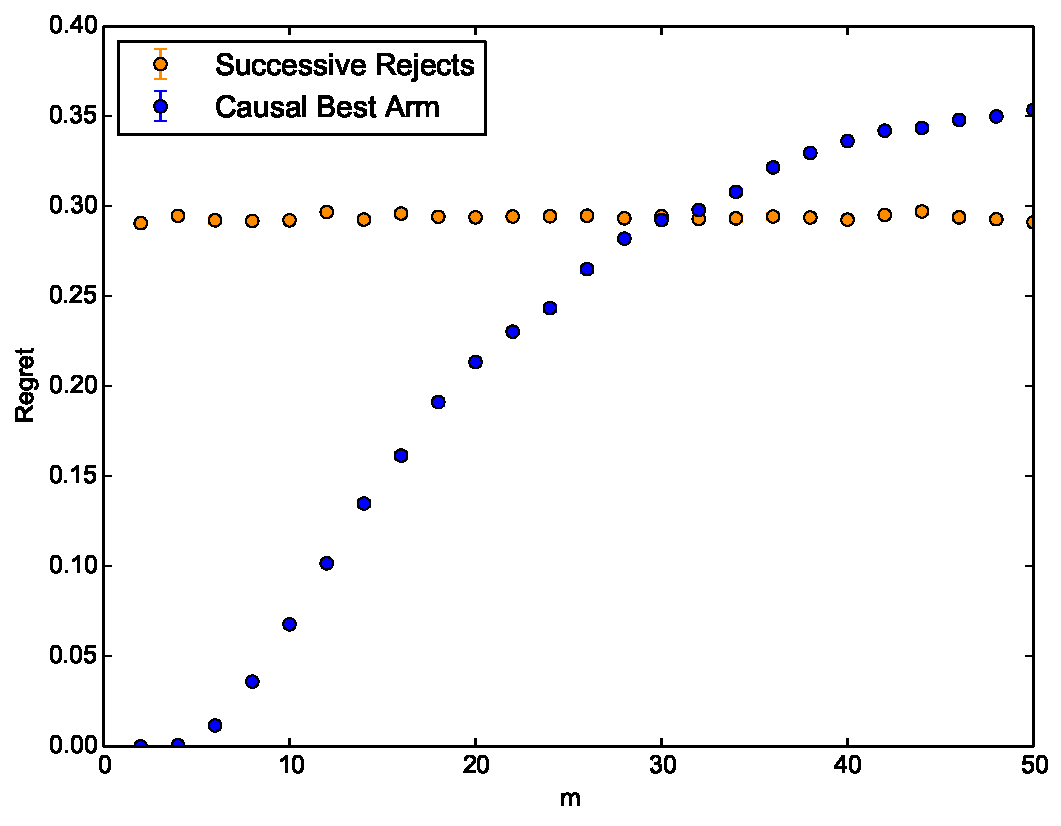
\includegraphics[width=.5\textwidth]{exp_simpleregret_vs_m_T300_N50_sims10000_10000.pdf}
\end{figure}

If figures \ref{fig:simple_vs_T_vary_epsilon} and \ref{fig:simple_vs_T} we compare the performance as a function of $T$. \todof{finish this}

For the parallel bandit problem, the regression estimator used in the specific algorithm outperforms the truncated importance weighted estimator in the more 
general algorithm, despite the fact the specific algorithm must estimate $\boldsymbol{q}$ from the data. 
This is an interesting phenomenon that has been noted before in off-policy evaluation where the regression (and not the importance weighted) estimator
is known to be minimax optimal asymptotically \citep{LMS14}.

\begin{figure}
\caption{Simple regret vs horizon, $T$, with $N = 50$ and $\epsilon = \sqrt{K/4T}$}
\label{fig:simple_vs_T_vary_epsilon}
\centering
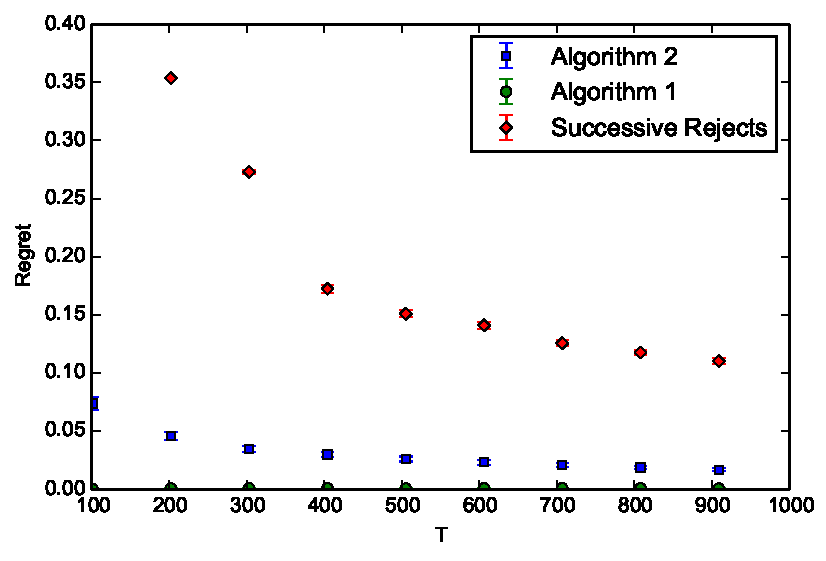
\includegraphics[width=.5\textwidth]{exp_regret_vs_T_N50_a4_s10000_20160204_1831}
\end{figure}

\begin{figure}
\caption{Simple regret vs horizon, $T$, with $N = 50$ and fixed $\epsilon = .3$}
\label{fig:simple_vs_T}
\centering
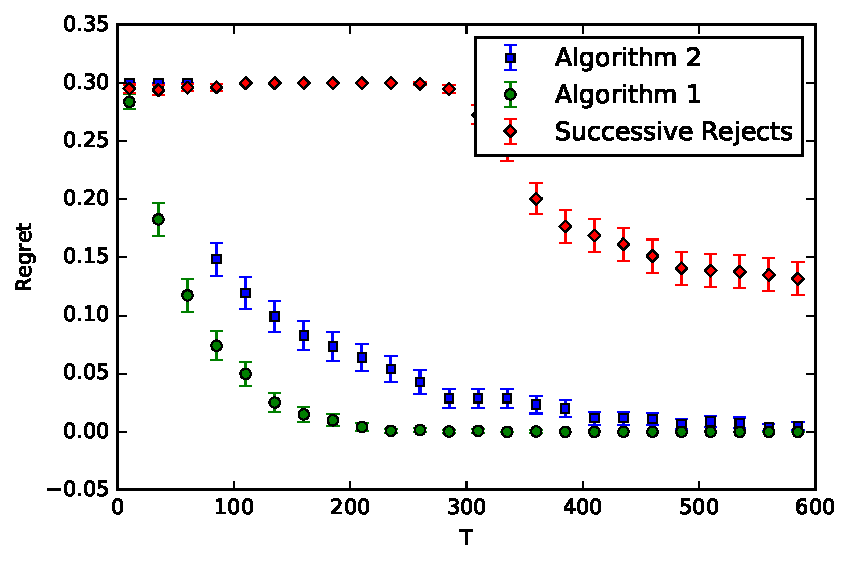
\includegraphics[width=.5\textwidth]{exp_regret_vs_T_N50_a4_s1000_20160205_1155}
\end{figure}


\subsection{Highly confounded problem}

 
\begin{figure}[h]
\centering
\caption{Causal model for the highly confounded problem.}
\label{fig:causalStructure_highly_confounded}
\begin{tikzpicture}[->,>=stealth',shorten >=1pt,auto,node distance=1cm,
  thick,main node/.style={observed}, hidden/.style={empty}]
\node[main node](1){$V_{2}$};
\node[main node, right=of 1](2){$X_{3}$};
\node[hidden, right=of 2](3){$...$};
\node[main node, right=of 3](4){$X_{N}$};
\node[main node, below right=of 2](5){Y};
\node[main node,above right=of 2](6){$X_1$}; 
 \path[every node/.style={font=\sffamily\small}]
    (1) edge (5)
    	(2) edge (5)
    (4) edge (5)
    (6) edge (1) edge (2) edge (4);
\end{tikzpicture}
\end{figure}


A model under which the value of the confounding variable $X_1$ plays the central role in determining $P(Y)$.  Let:
\eq {
\P{Z = 1} &= q \\
\P{X_k = 1|Z=j} &=  q_j \;\; \forall k \in \set{1...n}\\
\P{Y|x_1 ... x_n} &= \bar{\boldsymbol{x}}
} 
This leads to rewards:
\eq {
\P{Y|do(Z = j)} = q^j(1-q)^{1-j}\\
\P{Y|do(X_i = j)} = \begin{cases}
\frac{1}{n} + \frac{n-1}{n}\left(q q_1 + (1-q)q_0 \right) & \text{ if } j = 1 \\
\frac{n-1}{n}\left(q q_1 + (1-q)q_0 \right) & \text { if } j = 0
\end{cases}
}



